The top production cross-section is substantially higher with respect to the 
$\WW$ cross-section, and represents a significant challenge for studies of 
$\WW$ final states, including $H \to \WW$ searches. 
As explained in Section~\ref{sec:sel_toptag}, we use a dedicated top tagging 
veto, which allows to further suppress the top background. In addition, we use 
$b$-tagged events to determine the remaining top background. Details of the jet 
fragmentation cannot be reliably simulated at low energy, so the background 
should be estimated mainly from data.

The tagging methods have a significant tagging efficiency dependence on the jet 
$\pt$ threshold. Therefore, to reliably estimate the remaining top background 
we should estimate the tagging efficiency from a data control sample with 
similar properties as the data signal sample. Due to this feature, the method 
to extract the background depends on the corresponding jet bin. Another small 
complication is the fact that the $\ttbar$ and $tW$ processes show slightly 
different b-tagging behavior, although the difference can be taken as a small 
systematic uncertainty.

\subsubsection{0-Jet Bin Top Background Estimation}
To measure the top tagging efficiency after the jet veto we use top events 
with only one reconstructed jet as a control sample. In principle we can apply 
b-tagging to the reconstucted jet to increase the purity of the sample. The 
other b-quark can be tagged with the top tagging algorithm in hands. For the 
0-jet tt events the tagging efficiency should be 
$\epsilon_{2b} = 1 - (1-\epsilon_{1b})^2$, where $\epsilon_{2b}$ is the tagging 
efficiency for $\ttbar$ events that passed the jet veto and $\epsilon_{2b}$ is 
the tagging efficiency for top events with one jet, excluding the 
reconstructed jet from the top tagging algorithm.

The tagging efficiency for low $\pt$ jets, soft muon tagging efficiency 
and the combination of both of them as a function of the number of reconstructed 
jets in top events after applying the $\WW$-like selection are shown in 
Figure~\ref{fig:btag_njets_lowpttagging}. The tagging efficiency for low 
$\pt$ jets in the 1-jet bin is ($35 \pm 1$)\%, which gives an expected efficiency 
in the 0-jet bin of ($57 \pm 2$)\%. This is consistent with the obtained value 
in the 0-jet bin of ($53 \pm 4$)\%.

In addition, we measure the soft muon tagging efficiency in events with at least 
two reconstructed jets, which is a sample completely dominated by top events. 
The soft-muon tagging efficiency is about 20\%, with some decrease for low 
reconstructed jet bins. We can assume that the decrease is well-reproduced by 
the simulation since this is something expected to have.

\begin{figure}[!htbp]
\begin{center}
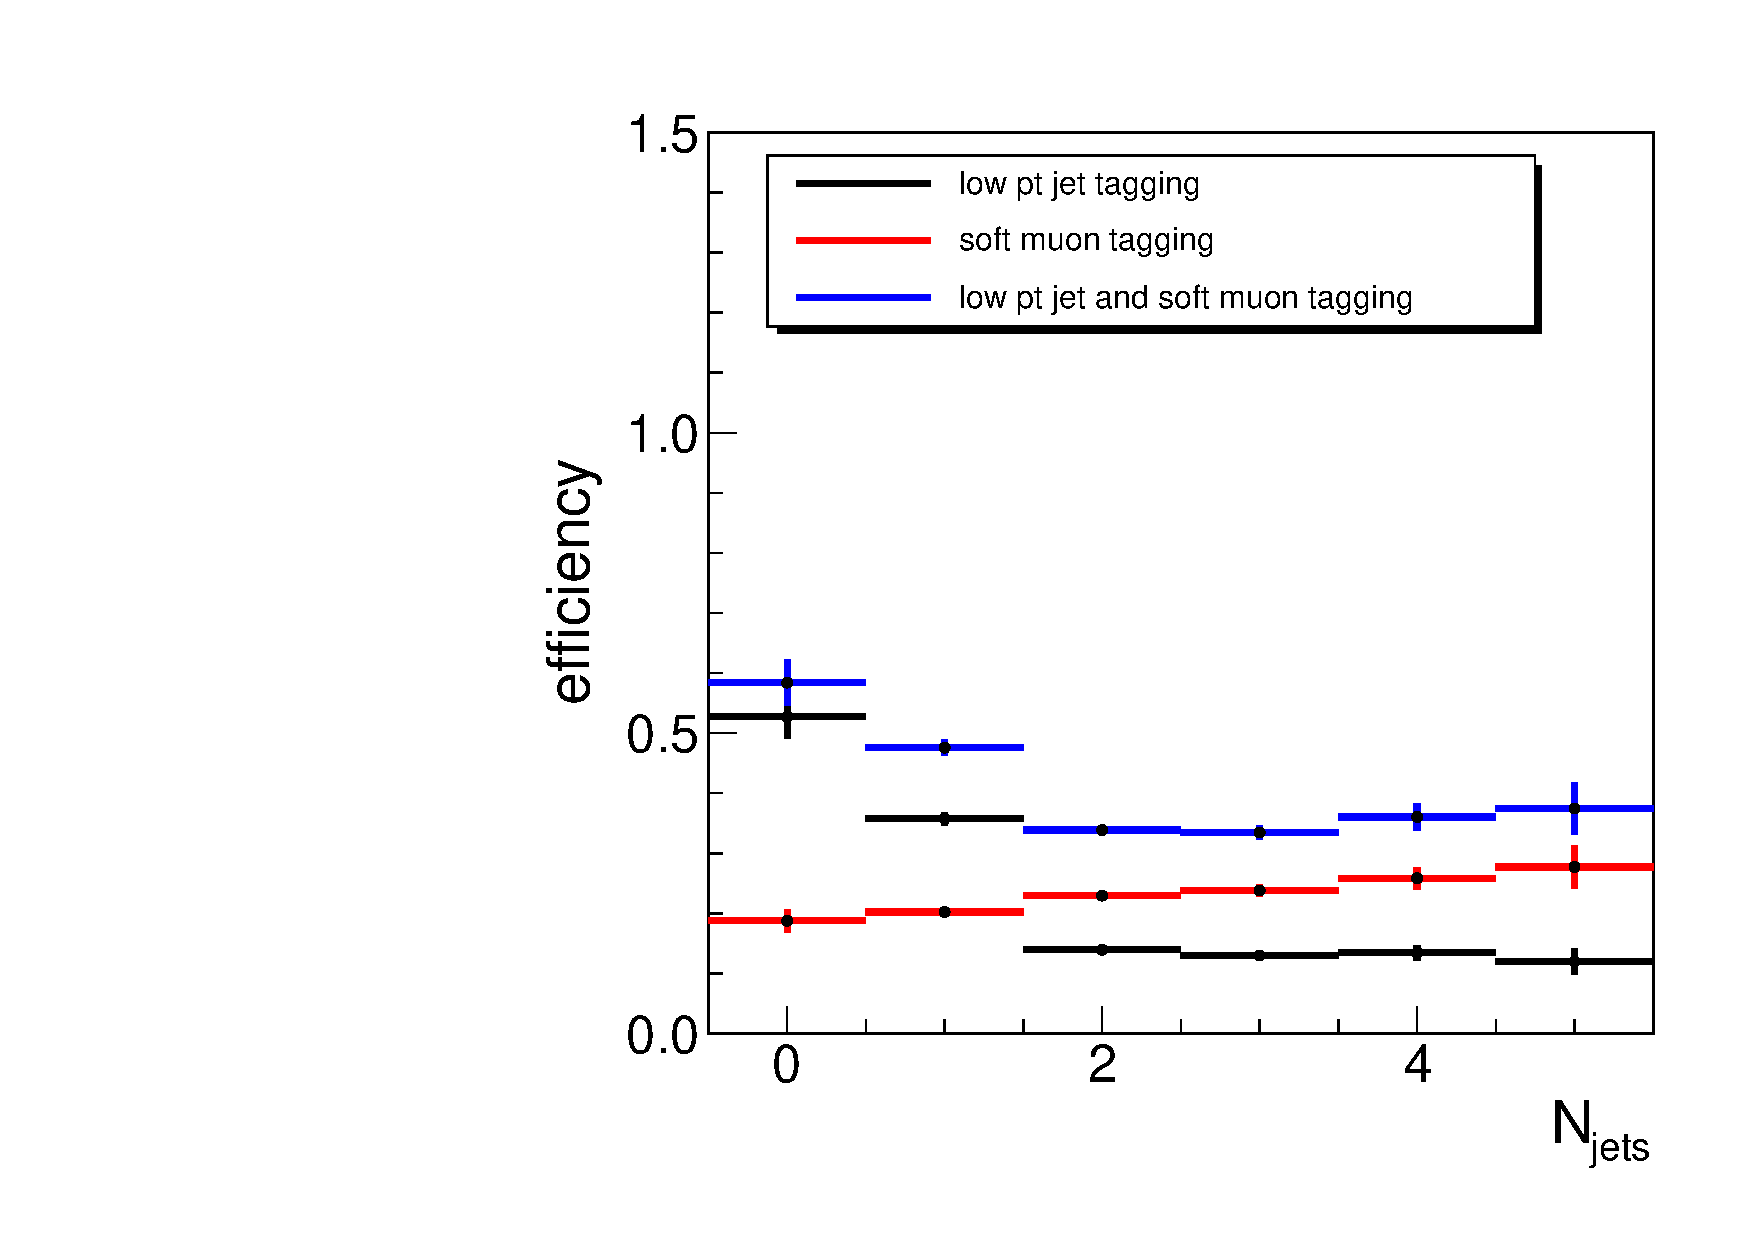
\includegraphics[width=0.55\textwidth]{figures/btag_njets_lowpttagging.pdf}
\caption{Tagging efficiency for low $\pt$ jets, soft muon tagging efficiency 
and the combination of both of them as a function of the number of reconstructed 
jets in top events after applying the $\WW$-like selection.}
\label{fig:btag_njets_lowpttagging}
\end{center}
\end{figure}

\subsubsection{1-Jet Bin Top Background Estimation}
To measure the top tagging efficiency in the jet 1-bin we use top events 
with two reconstructed jets as a control sample. The total 
tagging efficiency, where all jets and 
soft-muons are used, and tagging efficiency for the highest $\pt$ jet as a 
function of the number of reconstructed jets in top events after applying the 
$\WW$-like selection are shown in Figure~\ref{fig:btag_njets_highestptjet}.

Since there are kinematical differences among the jets for the different jet 
bins, there is some dependence in the total tagging efficiency. Nevertheless, 
the tagging efficiency for the highest $\pt$ jet in the event is approximately 
the same for the 1-jet and 2-jet bins, and it does not depend on the topology of
the other jets, as seen in Figure~\ref{fig:btag_njets_highestptjet}. Therefore, 
we propose to use events in the 2-jet bin to measure such efficiency.

\begin{figure}[!htbp]
\begin{center}
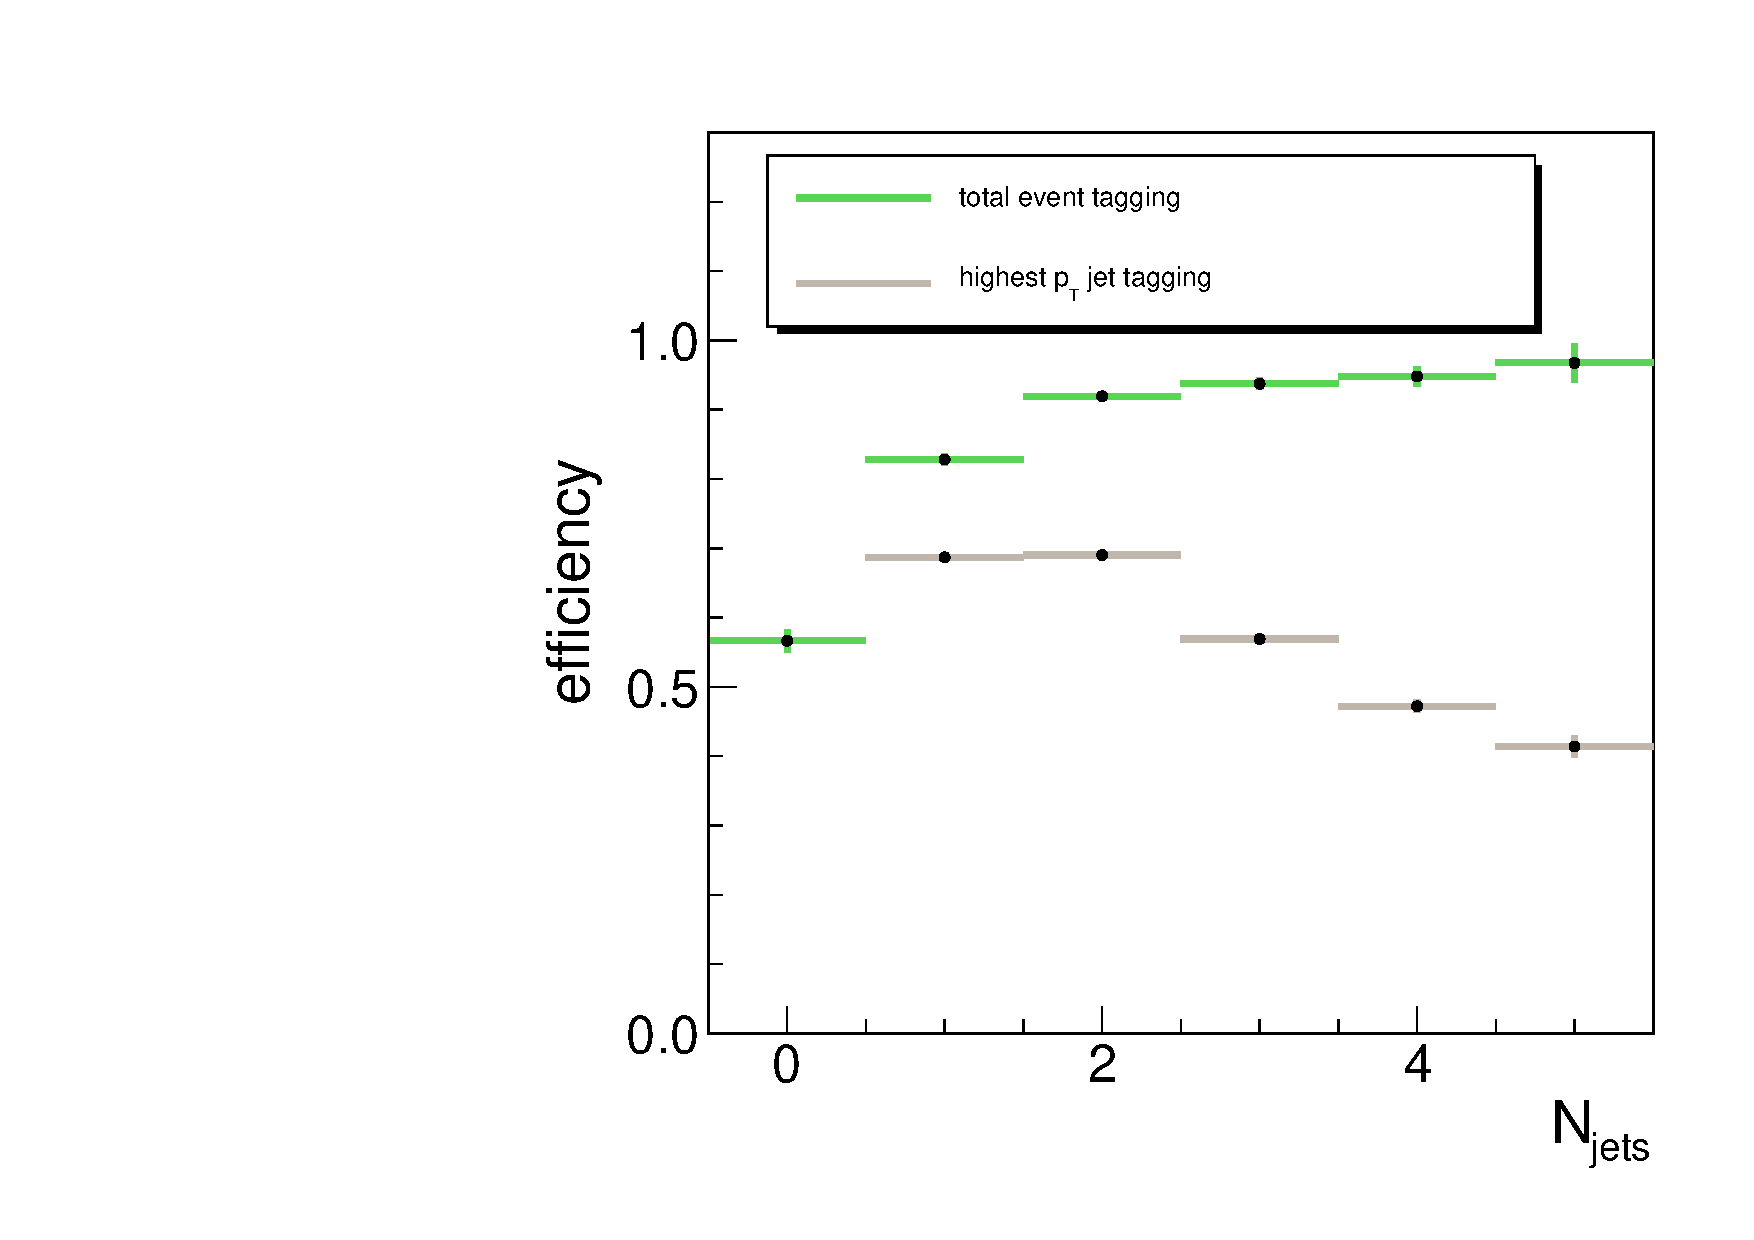
\includegraphics[width=0.55\textwidth]{figures/btag_njets_highestptjet.pdf}
\caption{Total tagging efficiency and tagging efficiency for the highest 
$\pt$ jet as a function of the number of reconstructed 
jets in top events after applying the $\WW$-like selection.}
\label{fig:btag_njets_highestptjet}
\end{center}
\end{figure}

In summary the number of top events in the 1-jet bin ($N_{no~tagged}^{1-jet}$) 
are estimated using tagged events with the highest $\pt$ jet 
($N_{tagged}^{1-jet}$) and its efficiency, as measured using the 2-jet bin
($\epsilon_{highest~\pt~jet}$): 
$N_{no~tagged}^{1-jet} = N_{tagged}^{1-jet} 
(1-\epsilon_{highest~\pt~jet})/\epsilon_{highest~\pt~jet}$. The closure test 
with simulated events give us an agreement well within the statistical 
uncertainty.
 
\subsubsection{2-Jet Bin Top Background Estimation}
The complication of the 2-jet bin is the additional jet requirements to select
the qqH-like events. As an example, we measure in simulated events the tagging
efficiency applying the following requirements: $\Delta \eta_{j1j2}>4$,
$m_{j1j2}>500~\GeVcc$ and $\eta_{j1}\eta_{j2}<0$. The total tagging efficiency 
and tagging efficiency for the highest $\pt$ jet as a function of the number 
of reconstructed jets in top events after applying such selection is shown in 
Figure~\ref{fig:btag_njets_vbfcuts}. In spite of the much lower of available
simulated events, the trend towards lower efficiency in the 2-jet bin, when
compared with the shown values in Figure~\ref{fig:btag_njets_highestptjet}, is
consistent with the expectation.

\begin{figure}[!htbp]
\begin{center}
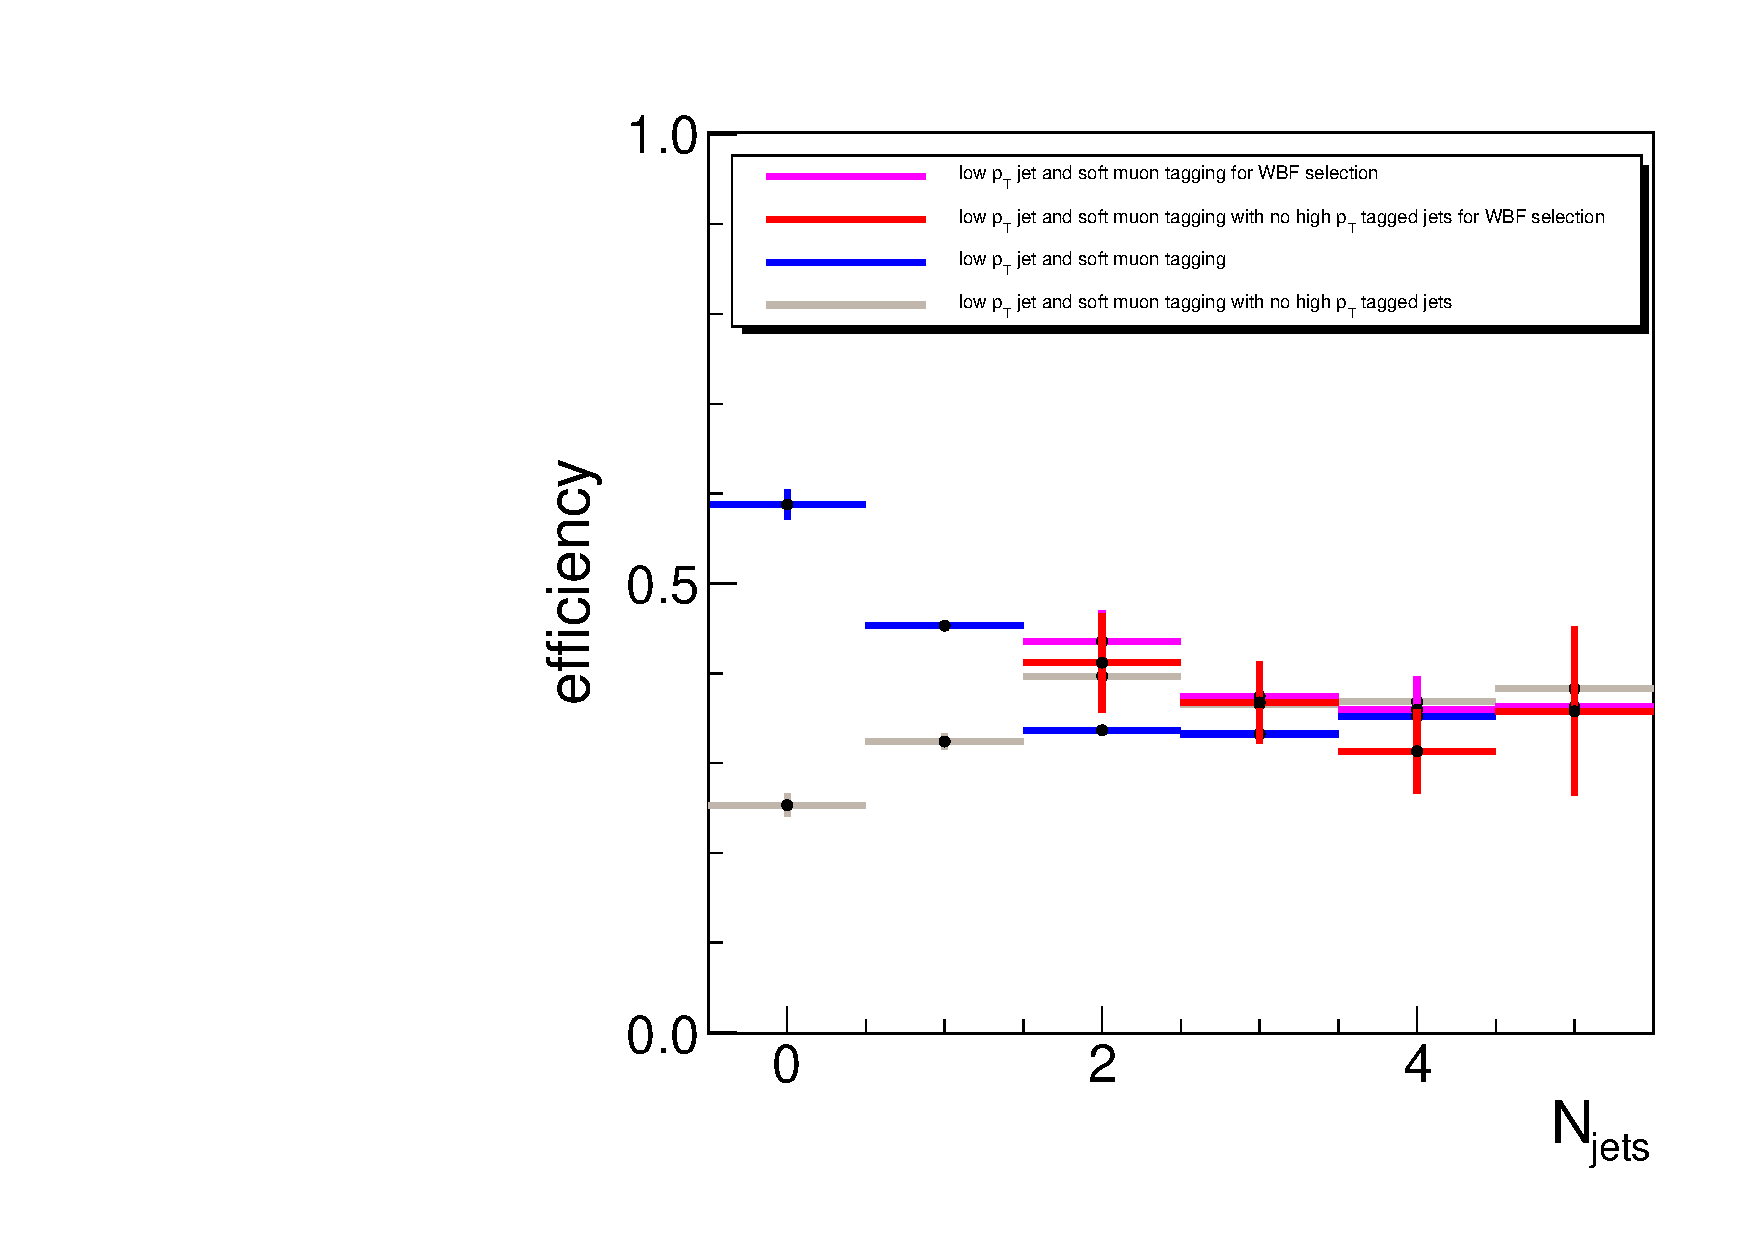
\includegraphics[width=0.55\textwidth]{figures/btag_njets_vbfcuts.pdf}
\caption{Total tagging efficiency and tagging efficiency for the highest 
$\pt$ jet as a function of the number of reconstructed 
jets in top events after applying the $\WW$-like selection and a qqH-like selection.}
\label{fig:btag_njets_vbfcuts}
\end{center}
\end{figure}

The proposed method is to measure the tagging efficiency for the leading and 
trailing jet as a function of $\eta$ and $\pt$ of its jet. This efficiency is
applied to untagged simulated top events. The tagging efficiency for low 
$\pt$ jets and soft muons is also measured from data.

\subsubsection{Top Background Estimation On Data}
The efficiency results on data after the subtraction of the background and the 
comparison with the prediction from the simulation, after applying the 
$\WW$-like selection, are summarized in this section. 
The tagging efficiency the combination for low $\pt$ jets and soft muons 
as a function of the number of reconstructed jets on data and 
simulation is shown in Figure~\ref{fig:btag_njets_lowpttagging_data}. The total 
tagging efficiency as a function of the number of reconstructed jets on data 
and simulation is shown in Figure~\ref{fig:btag_njets_totaltagging_data}. 
The tagging efficiency for the leading jet $\pt$ as a function of the number of 
reconstructed jets on data and simulation is shown in 
Figure~\ref{fig:btag_njets_highestptjet_data}. In all cases a reasonable agreement 
is found between the data result and the prediction from the simulation, although the 
statistical uncertainty is still very large

\begin{figure}[!htbp]
\begin{center}
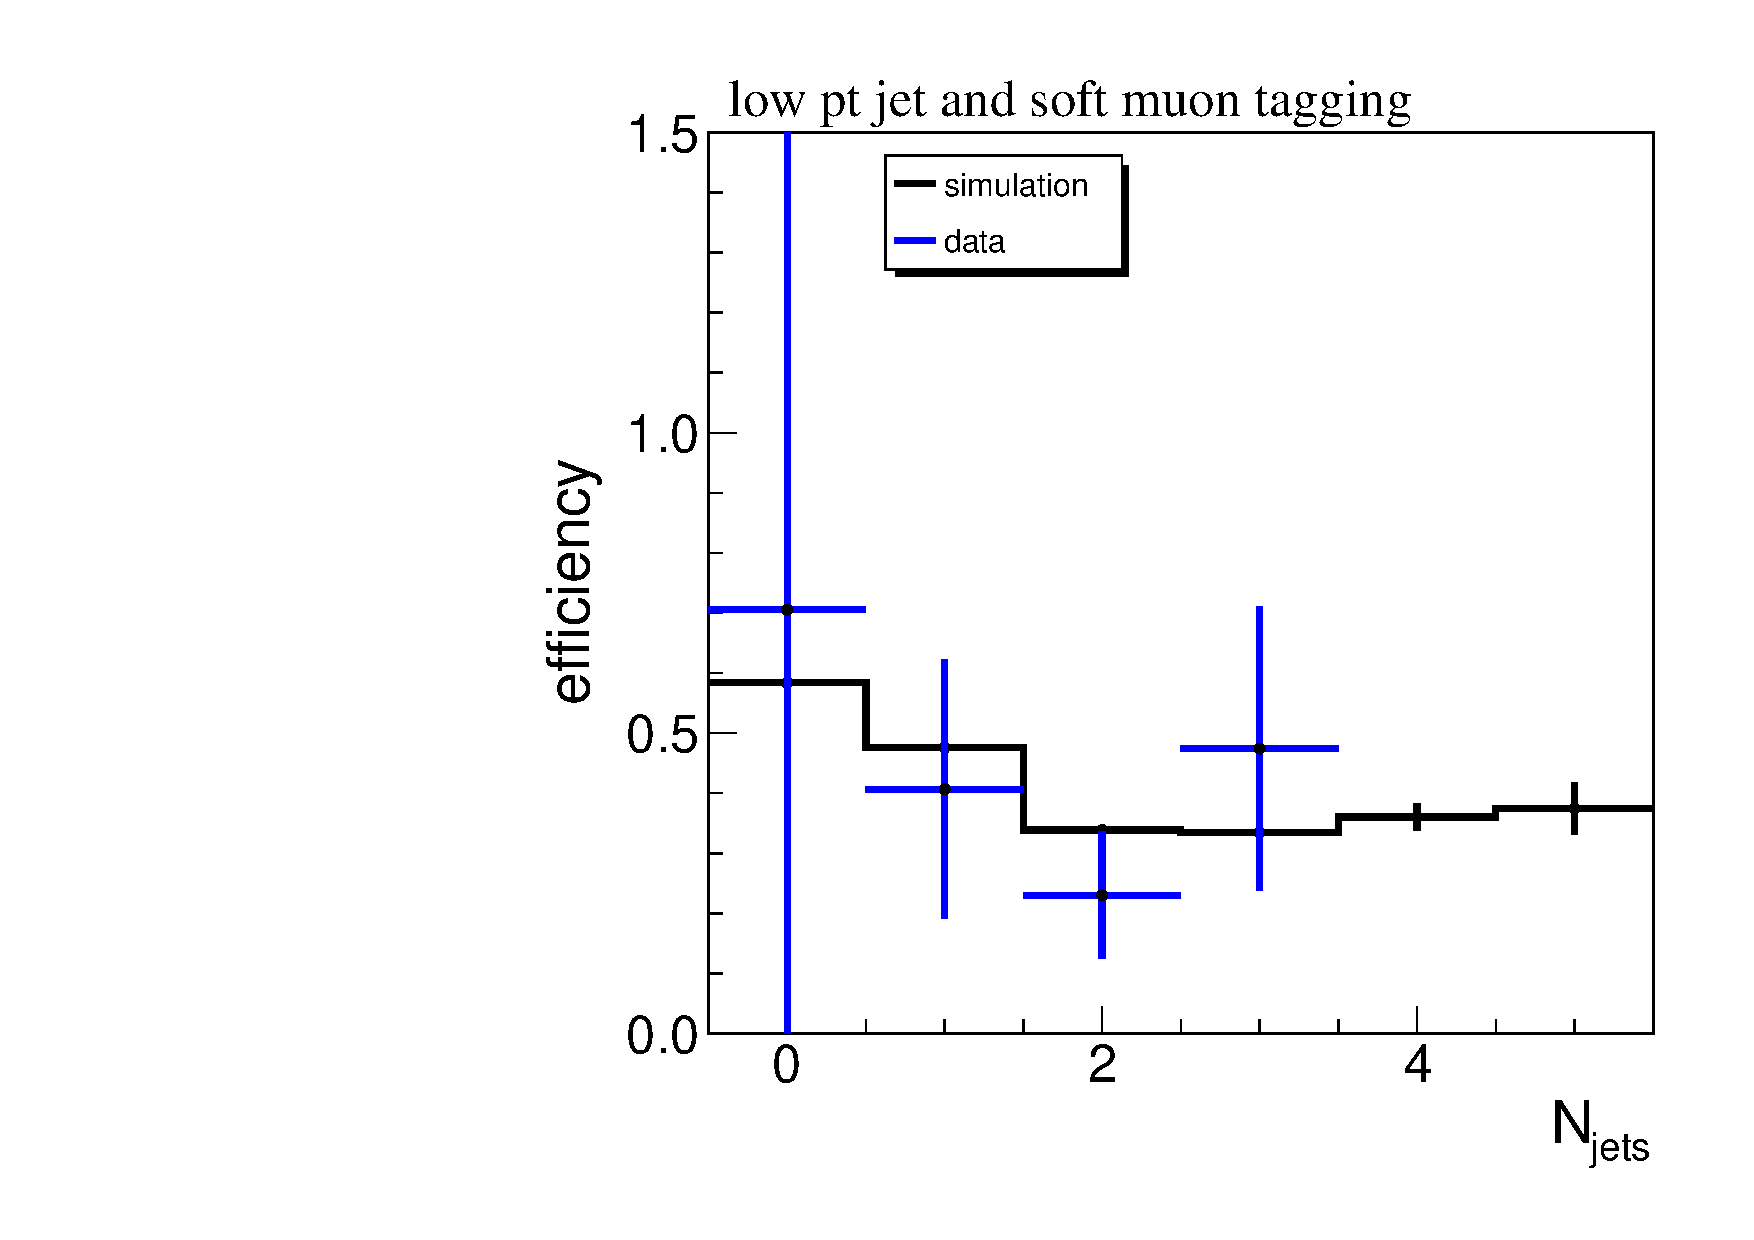
\includegraphics[width=0.55\textwidth]{figures/btag_njets_lowpttagging_data.pdf}
\caption{Tagging efficiency the combination  for low $\pt$ jets and soft muons 
as a function of the number of reconstructed jets after applying 
the $\WW$-like selection on data and simulation.}
\label{fig:btag_njets_lowpttagging_data}
\end{center}
\end{figure}

\begin{figure}[!htbp]
\begin{center}
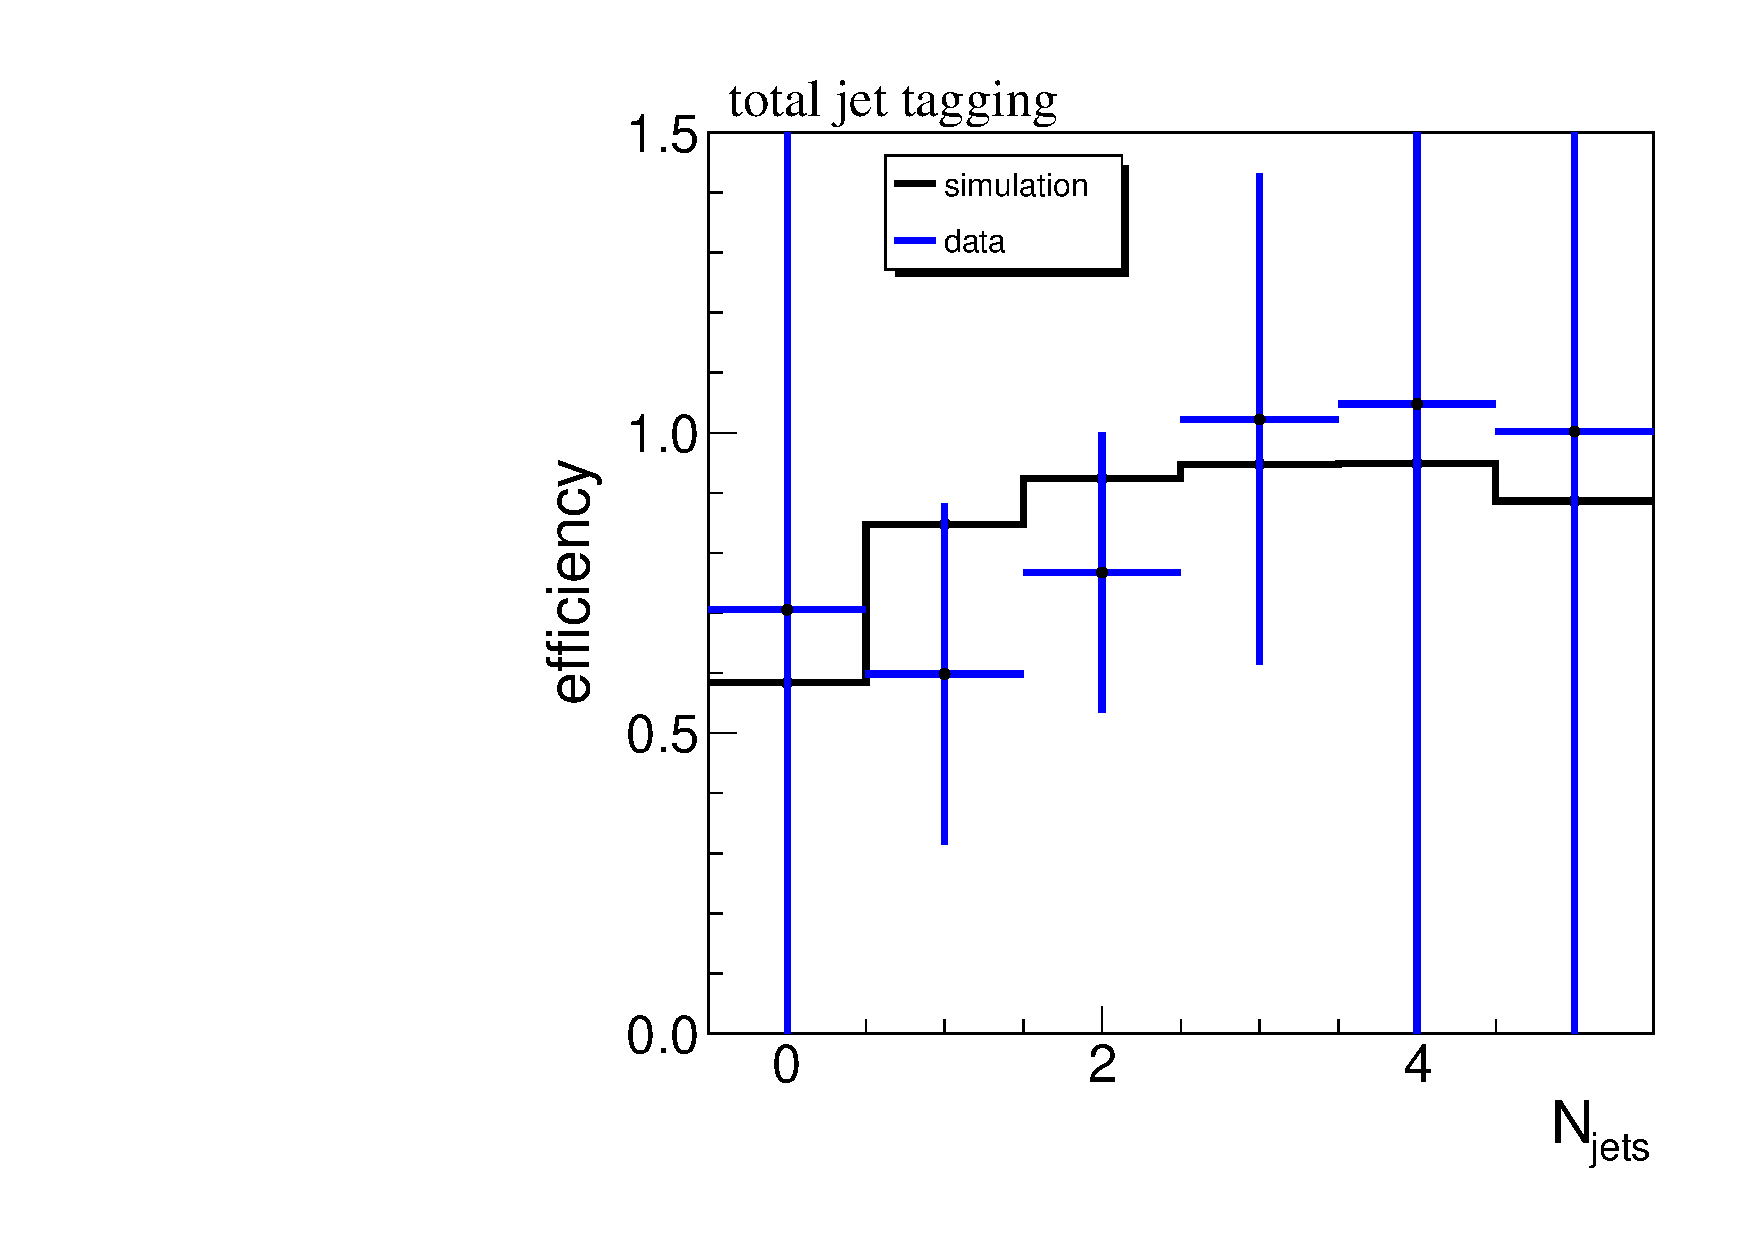
\includegraphics[width=0.55\textwidth]{figures/btag_njets_totaltagging_data.pdf}
\caption{The total tagging efficiency as a function of the number of reconstructed 
jets after applying the $\WW$-like selection on data and simulation.}
\label{fig:btag_njets_totaltagging_data}
\end{center}
\end{figure}

\begin{figure}[!htbp]
\begin{center}
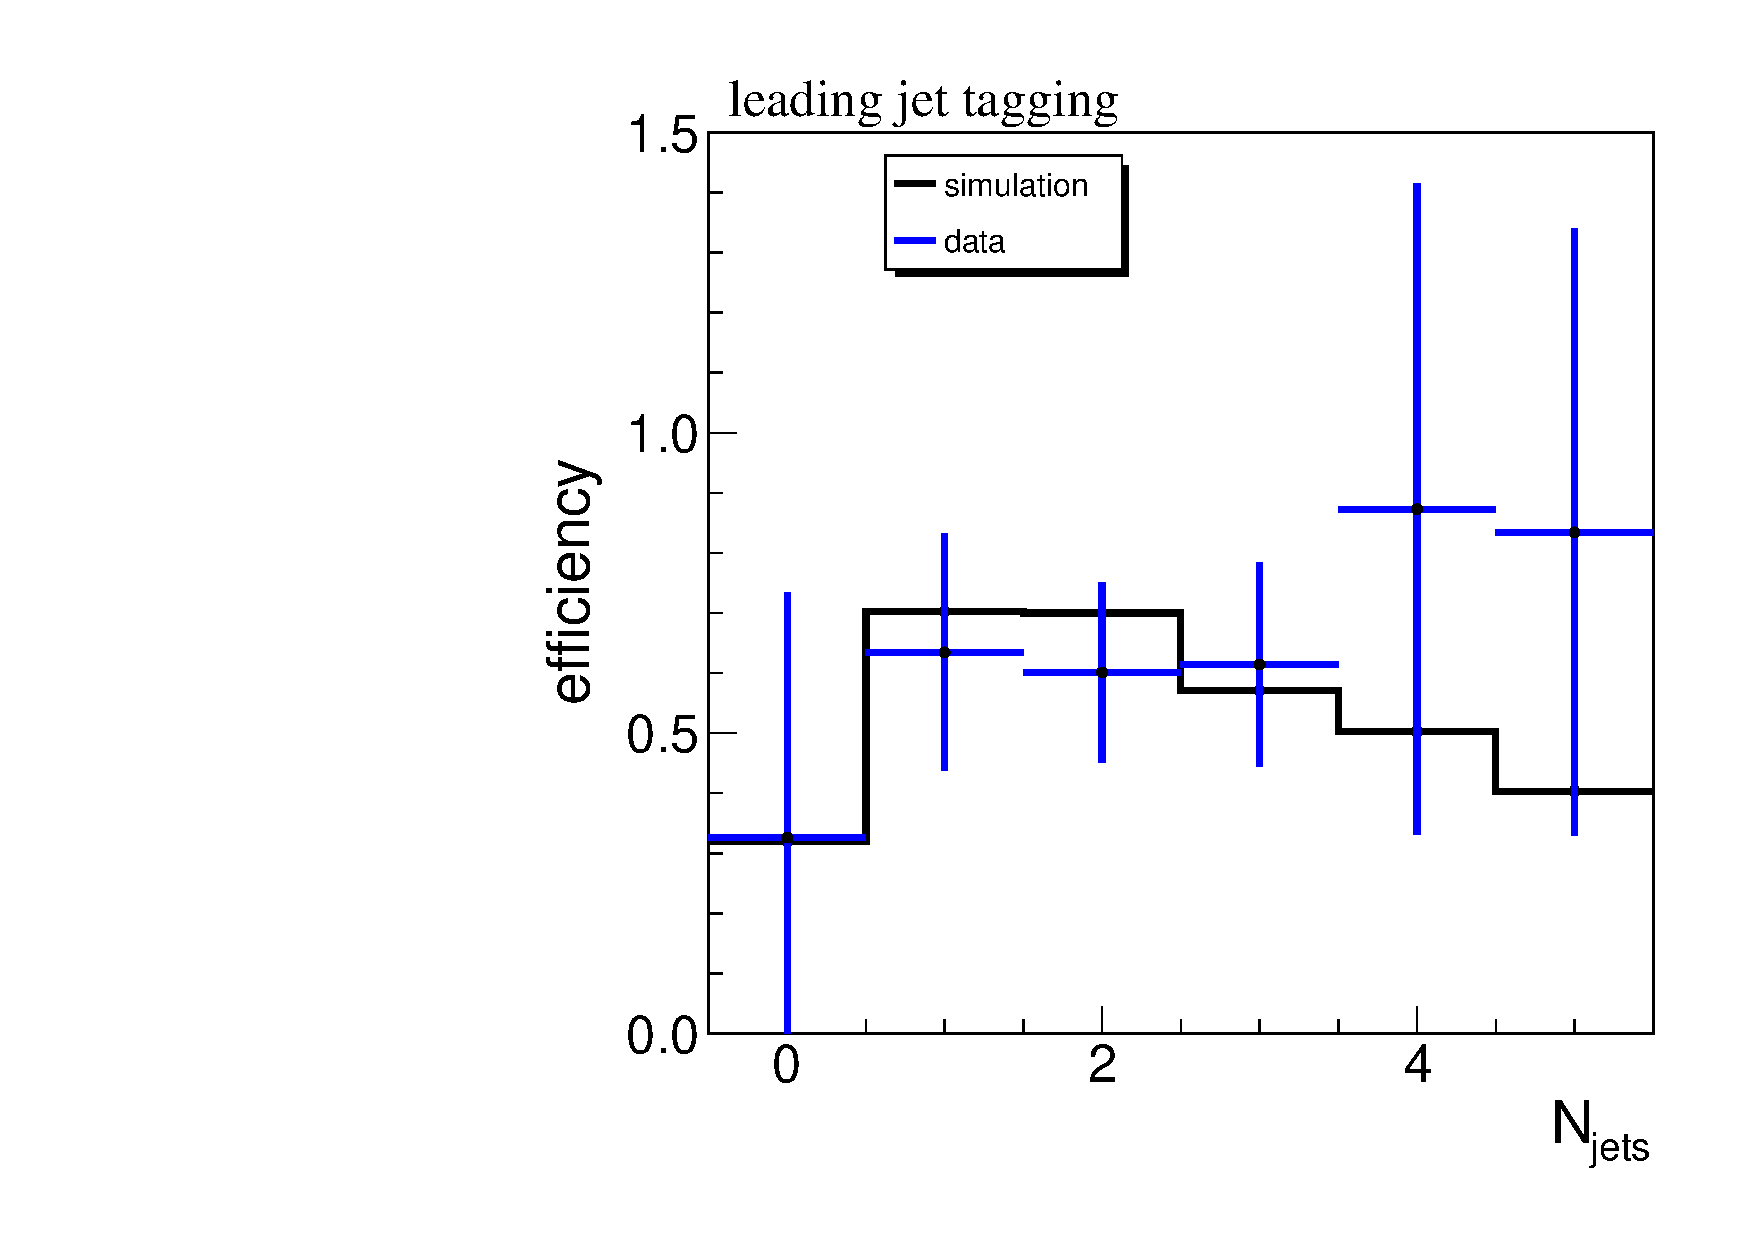
\includegraphics[width=0.55\textwidth]{figures/btag_njets_highestptjet_data.pdf}
\caption{Tagging efficiency for the leading jet $\pt$ as a function of the number of reconstructed 
jets after applying the $\WW$-like selection on data and simulation.}
\label{fig:btag_njets_highestptjet_data}
\end{center}
\end{figure}

